\chapter[Análisis cuantitativo de trayectorias]{Análisis cuantitativo\\de trayectorias}
\label{chap:analisis-trayectorias}

Este capítulo describe los cálculos aplicados a las trayectorias reconstruidas: distancias, rapidez, variaciones temporales e indicadores de actividad. Se precisan las referencias temporales, las unidades y las decisiones de implementación que condicionan su interpretación. La descripción corresponde al procesamiento actual en píxeles y a los parámetros operativos del sistema.

\section{Referencia temporal y duración}

El parámetro \texttt{analysis\_fps}, denotado aquí por $F$, configura la conversión temporal definida en el capítulo 2. Su valor predeterminado es $30$ cuadros/s y no se obtiene automáticamente del video. Debe identificarse en cada ejecución y distinguirse del FPS empleado al escribir el video de salida.

El cálculo de duración e intervalos conserva la separación entre los índices registrados, incluidos los gaps descritos en el capítulo~\ref{chap:seguimiento}. Las funciones temporales verifican el orden de las observaciones y rechazan frecuencias no positivas. Los gráficos usan por defecto el tiempo del video para ubicar cada trayectoria dentro de la grabación.

\section{Coordenadas y unidades de medida}

El procesamiento conserva las coordenadas del seguimiento en píxeles. Las salidas actuales expresan posiciones y distancias en px, rapidez en px/s y variación de rapidez en px/s$^2$. Los indicadores de rectitud e inactividad son adimensionales.

\subsection{Alcance de las unidades espaciales}

Los resultados describen el movimiento en el plano de la imagen. Su conversión a micrómetros requeriría una calibración externa del sistema óptico, bajo las mismas condiciones de adquisición. Esa etapa está fuera del alcance del trabajo y no se incorpora al procesamiento ni a la evaluación presentada.

\section{Distancias y rectitud de la trayectoria}

Se utilizan las definiciones geométricas del capítulo 2. Para cada par de observaciones consecutivas se calcula la norma euclidiana de la diferencia de posiciones. Su suma proporciona la distancia acumulada $D_T$, mientras que la distancia neta $D_N$ es la norma del desplazamiento entre la primera y la última posición. Ambas magnitudes describen el registro bidimensional disponible.

El cálculo incluye el segmento que une dos observaciones separadas por un gap. Esa contribución mide la separación entre sus extremos, sin recuperar el recorrido realizado durante los cuadros ausentes. Por ello, la suma de segmentos no debe interpretarse como una reconstrucción completa del movimiento continuo. Los errores de localización también pueden aumentar la longitud acumulada mediante fluctuaciones de posición.

El índice de rectitud se obtiene como $S=D_N/D_T$, cuando $D_T>0$. Un valor próximo a uno indica que el desplazamiento entre extremos representa una proporción alta de la longitud acumulada. Un valor reducido puede aparecer en recorridos con retornos o cambios de dirección; por sí solo no identifica un tipo de movimiento. Si $D_T=0$, la función de rectitud devuelve un valor no definido y el resumen de trayectorias omite ese caso en su ordenamiento por rectitud.

Esta propiedad geométrica se distingue de la continuidad temporal del capítulo~\ref{chap:seguimiento}. Una trayectoria con gaps puede ser rectilínea, y otra registrada en cuadros consecutivos puede presentar un recorrido curvo.

La Figura~\ref{fig:distancias-trayectoria} ilustra estas magnitudes con las posiciones conservadas de \texttt{Track\_145}. El recorrido acumulado incluye sus cambios de dirección, mientras que el segmento entre inicio y fin representa únicamente el desplazamiento neto. El ejemplo se utiliza aquí para mostrar el cálculo geométrico; su evaluación experimental se desarrolla en el capítulo~\ref{chap:evaluacion-resultados}.

\begin{figure}[H]
  \centering
  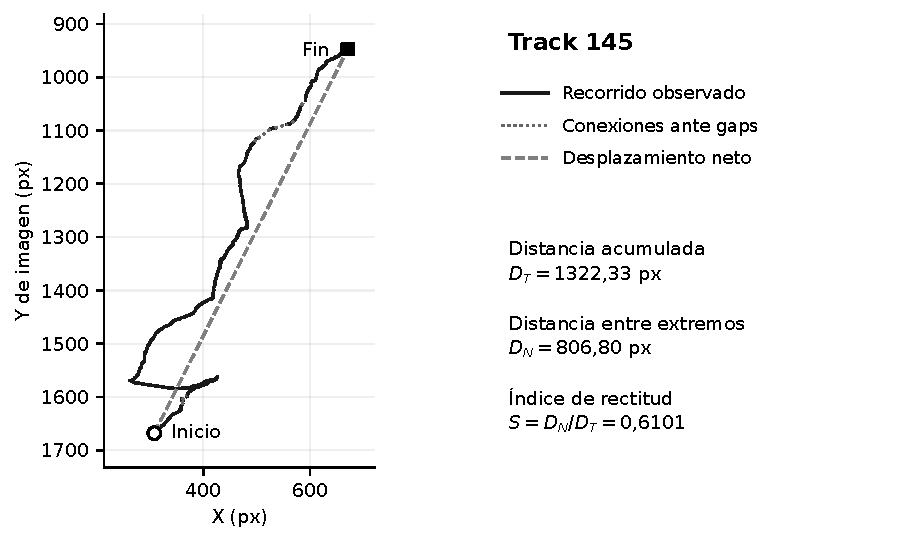
\includegraphics[width=0.90\textwidth]{figures/chapter08/fig08_01_distancias_trayectoria.pdf}
  \caption{Distancia acumulada ($D_T$), distancia entre extremos ($D_N$) y rectitud ($S$) de \texttt{Track\_145}, calculadas sobre sus 929 observaciones. El círculo indica el inicio y el cuadrado, el fin. Los tramos punteados conectan observaciones separadas por gaps y contribuyen a $D_T$ mediante la separación entre sus extremos; la línea discontinua representa $D_N$. Los ejes conservan la misma escala espacial y la orientación vertical de la imagen.}
  \label{fig:distancias-trayectoria}
\end{figure}

\section{Rapidez y suavizado temporal}

\subsection{Rapidez por segmento y promedios}

Para $n\geq2$ observaciones, la rapidez de cada segmento se calcula como
\begin{equation}
  v_i=\frac{\lVert\vec{p}_{i+1}-\vec{p}_i\rVert}{\Delta t_i},
  \qquad \vec{p}_i=(x_i,y_i),\quad i=1,\ldots,n-1.
  \label{eq:rapidez-segmento-implementada}
\end{equation}
El resultado se asocia con el cuadro final $f_{i+1}$. Es una estimación escalar sobre el intervalo entre posiciones observadas, no una medición instantánea de todo el movimiento ocurrido en su interior. Aunque algunas interfaces utilicen la palabra \emph{velocidad}, aquí se emplea \emph{rapidez} para conservar esta distinción.

La inspección individual conserva dos promedios distintos:
\begin{equation}
  \overline{v}_{\mathrm{seg}}=\frac{1}{n-1}\sum_{i=1}^{n-1}v_i,
  \qquad
  \overline{v}_{\mathrm{tray}}=\frac{D_T}{T}
  =\frac{\sum_i v_i\Delta t_i}{\sum_i\Delta t_i}.
  \label{eq:promedios-rapidez}
\end{equation}
El primero asigna el mismo peso a cada segmento; el segundo pondera por su duración. Coinciden cuando los intervalos son iguales, pero pueden diferir ante gaps. Se exponen, respectivamente, como \texttt{mean\_segment\_speed} y \texttt{trajectory\_average\_speed}; el campo de compatibilidad \texttt{avg\_speed} conserva la primera interpretación.

La Figura~\ref{fig:promedios-rapidez} ilustra esa diferencia con tres observaciones en los cuadros $0$, $1$ y $4$, separadas espacialmente por $10$ px en cada segmento. Con $F=30$, se obtienen $300$ y $100$ px/s: su media aritmética es $200$ px/s, mientras que $D_T/T=20/(4/30)=150$ px/s.

\begin{figure}[htbp]
  \centering
  \begin{tikzpicture}[x=1.1cm,y=0.85cm]
    \draw[thesisarrow] (0,0) -- (4.7,0);
    \draw[thesisarrow] (0,0) -- (0,3.7);
    \node[font=\small] at (2.5,-0.85) {Tiempo del video (s)};
    \node[font=\small,rotate=90] at (-0.9,1.9) {Rapidez (px/s)};
    \foreach \y/\v in {1/100,1.5/150,2/200,3/300} {
      \draw (-0.06,\y) -- (0.06,\y);
      \node[font=\small,anchor=east] at (-0.13,\y) {$\v$};
    }
    \foreach \x/\t in {0/0,1/{0{,}033},4/{0{,}133}} {
      \draw (\x,-0.06) -- (\x,0.06);
      \node[font=\small,anchor=north] at (\x,-0.15) {$\t$};
    }
    \draw[dashed] (0,2) -- (4.4,2);
    \draw[densely dotted] (0,1.5) -- (4.4,1.5);
    \fill (1,3) circle (2.5pt);
    \fill (4,1) circle (2.5pt);
    \node[font=\small,anchor=west] at (4.6,3) {Rapidez por segmento};
    \node[font=\small,anchor=west] at (4.6,2) {$\overline{v}_{\mathrm{seg}}=200$ px/s};
    \node[font=\small,anchor=west] at (4.6,1.5) {$\overline{v}_{\mathrm{tray}}=150$ px/s};
  \end{tikzpicture}
  \caption{Ejemplo numérico ilustrativo de los dos promedios de rapidez. Los puntos representan valores por segmento asociados con sus cuadros finales; las líneas horizontales indican promedios. Los tiempos se muestran redondeados. No corresponde a un resultado experimental.}
  \label{fig:promedios-rapidez}
\end{figure}

\subsection{Media móvil y alineación temporal}

La rapidez se suaviza mediante una media móvil de $w$ valores consecutivos de la serie calculada. Si esta contiene $m=n-1$ segmentos, se obtiene
\begin{equation}
  \widetilde{v}_j=\frac{1}{w}\sum_{k=j}^{j+w-1}v_k,
  \qquad j=1,\ldots,m-w+1.
\end{equation}
La operación utiliza únicamente ventanas completas y asigna cada resultado al cuadro del último segmento incluido, $f_{j+w}$. Por tanto, genera $M=m-w+1$ valores cuando $m\geq w$; en caso contrario, devuelve una serie vacía. Con $w=20$ se requieren al menos 21 posiciones para obtener un valor suavizado.

La ventana cuenta muestras, no segundos ni cuadros necesariamente consecutivos. Su duración efectiva puede variar, y la media móvil puede combinar segmentos separados por gaps. El suavizado no divide automáticamente la trayectoria en bloques continuos. También reduce la resolución temporal de variaciones breves y puede desplazar su representación hacia el final de la ventana.

\section{Variación temporal de la rapidez}

Sobre la serie suavizada, el sistema estima diferencias de rapidez por unidad de tiempo. Si $g_j$ es el cuadro asociado con su muestra $j$, el cálculo es
\begin{equation}
  a_j=\frac{\widetilde{v}_{j+1}-\widetilde{v}_j}{(g_{j+1}-g_j)/F}.
  \label{eq:variacion-rapidez-implementada}
\end{equation}
La función utiliza las diferencias reales entre cuadros y requiere al menos dos valores de rapidez. La magnitud se expresa en px/s$^2$ y representa una variación escalar de rapidez. No reconstruye el vector de aceleración ni describe por sí sola cambios de dirección a rapidez constante.

Los gráficos señalan aumentos bruscos si $a_j>A$ y disminuciones bruscas si $a_j<-A$. Estas marcas se asignan a la muestra posterior de la diferencia. El umbral $A$ es operativo; las denominaciones de aceleración o frenada utilizadas en la visualización no establecen un mecanismo físico o biológico.

\section{Inactividad y cambios de régimen}

\subsection{Muestras bajo el umbral de actividad}

La condición de inactividad se aplica a la rapidez suavizada mediante $\widetilde{v}_j<u$. Cuando existen $M>0$ valores, la inspección calcula
\begin{equation}
  I=\frac{1}{M}\sum_{j=1}^{M}\mathbf{1}[\widetilde{v}_j<u].
  \label{eq:fraccion-inactividad}
\end{equation}
El resultado es una fracción entre cero y uno. El campo \texttt{inactivity\_percentage} almacena esa fracción, sin multiplicarla por cien. Sus términos cuentan muestras suavizadas, sin ponderarlas por duración. En consecuencia, no se interpreta directamente como la proporción del tiempo total durante la cual el microorganismo permaneció inmóvil.

La inspección conserva los cuadros finales asociados con las muestras que cumplen el criterio y sus tiempos en el video. El umbral identifica valores reducidos de rapidez según la configuración; no demuestra ausencia de movimiento durante todo el intervalo ni constituye un diagnóstico biológico de inactividad.

\subsection{Comparación entre ventanas de rapidez}

Los cambios de régimen se señalan comparando la media de $r$ muestras suavizadas previas con la de $r$ muestras a partir del punto evaluado. Se marca una posición interior cuando la diferencia absoluta entre esas medias alcanza o supera un umbral $\delta$. El recorrido de la serie excluye los extremos donde la implementación no realiza esa comparación.

El criterio puede marcar varias posiciones cercanas durante una transición, ya que no incorpora una consolidación posterior de eventos. Sus ventanas también se definen por cantidad de muestras y pueden abarcar gaps. Estas marcas describen diferencias entre niveles locales de rapidez; la clasificación del tipo de movimiento se desarrolla en el capítulo siguiente.

El Cuadro~\ref{tab:parametros-analisis-trayectorias} resume los parámetros operativos predeterminados, sin optimización experimental documentada. Las rutinas pueden omitir productos si no hay muestras suficientes para sus ventanas.

\begin{table}[htbp]
  \centering
  \small
  \caption{Parámetros operativos del análisis cuantitativo.}
  \label{tab:parametros-analisis-trayectorias}
  \begin{tabularx}{\textwidth}{@{}l l X@{}}
    \toprule
    Parámetro & Valor & Función \\
    \midrule
    $F$ & $30$ cuadros/s & Frecuencia utilizada para convertir cuadros a tiempo. \\
    $w$ & $20$ muestras & Ventana de la media móvil de rapidez. \\
    $u$ & $30$ px/s & Umbral de inactividad: comparación estricta por debajo. \\
    $A$ & $450$ px/s$^2$ & Umbral de variación brusca de rapidez. \\
    $r$ & $50$ muestras & Tamaño de cada ventana para cambios de régimen. \\
    $\delta$ & $30$ px/s & Diferencia mínima entre medias locales. \\
    \bottomrule
  \end{tabularx}
\end{table}

\section{Resúmenes y visualizaciones}

La inspección individual reúne posiciones, distancias, rapideces y muestras bajo el umbral de actividad. Sus gráficos muestran el recorrido bidimensional, las rapideces originales o suavizadas y las marcas de inactividad o cambio. Los límites del modo \texttt{context} ajustan la ventana visible alrededor de los datos sin reiniciar el origen temporal del video. La trayectoria individual se dibuja con el eje vertical invertido para conservar la orientación de la imagen, sin modificar las coordenadas almacenadas.

En las curvas temporales individuales se insertan interrupciones gráficas ante gaps de la serie y se sombrean sus intervalos. Esto no elimina los segmentos calculados sobre observaciones separadas ni impide que el suavizado abarque esos intervalos. La trayectoria espacial, en cambio, une posiciones consecutivas de la lista, incluso cuando sus cuadros no son consecutivos.

El resumen general ordena trayectorias por distancia acumulada, desviación estándar de las rapideces por segmento e índice de rectitud. La etiqueta de trayectorias más \emph{irregulares} utilizada en la salida se refiere a variabilidad de rapidez, no a irregularidad geométrica. El atributo histórico \texttt{n\_continuous} utiliza rectitud, no cobertura temporal; la corrección de etiquetas lo presenta como ranking de mayor rectitud. Se muestran hasta cinco ejemplos por criterio, según la configuración y la cantidad disponible.

Una función auxiliar permite graficar la media de rapideces agrupadas por el cuadro final de cada segmento. Ese promedio reúne solo los tracks con una rapidez asociada al cuadro correspondiente; no presupone un conjunto constante de individuos ni equivale a una media de trayectorias completas. Su disponibilidad se distingue de los productos activados por defecto en el procesamiento general.

\begin{samepage}
El ejemplo geométrico de la Figura~\ref{fig:distancias-trayectoria} ilustra la construcción y el significado de las distancias y la rectitud. La evaluación experimental y las comparaciones con referencias manuales se desarrollan en el capítulo~\ref{chap:evaluacion-resultados}.
\par
\end{samepage}

\section{Consideraciones y limitaciones}

Las métricas dependen de las posiciones, la identidad asignada por el seguimiento y los FPS de análisis. Una frecuencia incorrecta modifica la escala temporal de la rapidez y de sus variaciones. Los errores de localización pueden introducir fluctuaciones; los cambios de identidad pueden generar segmentos que mezclen individuos. El suavizado y los umbrales no garantizan la corrección de esos casos.

Los gaps se conservan en los intervalos temporales, pero no permiten conocer el recorrido intermedio. Las ventanas móviles y los promedios sin ponderación temporal deben interpretarse considerando esa disponibilidad desigual. Tampoco se equipara una rectitud elevada con seguimiento correcto o con una categoría de movimiento específica.

\begin{samepage}
Los valores no definidos y las series vacías deben distinguirse de resultados físicamente nulos. Algunas salidas de compatibilidad muestran cero cuando faltan rapideces; ese valor no demuestra estacionariedad. Asimismo, una trayectoria con pocos puntos puede devolver distancia acumulada nula sin contener observaciones suficientes para caracterizar el movimiento.
\par
\end{samepage}

En la revisión utilizada para reconstruir los resultados, la referencia relativa de la curva no se aplicaba a las marcas auxiliares de inicio, fin y gaps. La corrección de presentación utiliza los cuadros originales de las posiciones para incluir el gap inicial y expresa también las marcas auxiliares en la referencia elegida. Esa modificación conserva las muestras y los cálculos numéricos. La descripción principal de este capítulo utiliza el tiempo del video, que es la referencia predeterminada de los gráficos.

En la versión corregida de las visualizaciones operativas, las gráficas espaciales y las estelas de los videos individuales se interrumpen ante cuadros ausentes. Las conexiones punteadas del ejemplo geométrico de la Figura~\ref{fig:distancias-trayectoria} conservan un propósito distinto: ilustran la separación entre extremos que contribuye a la distancia acumulada, sin afirmar un recorrido observado durante el gap.
